\section{유한 온도 quotient와 인증된 재구성}
\subsection{온도 도함수를 같은 endpoint 식으로 읽기}
원 온도 정의는
\[
\ell_e=(1,f,2f,0),\quad \Pi(g)=1+f+\ell_eg,\quad
C_T=\frac{2\epsilon_{\rm eV}}{3k_B},\quad
T(g)=\frac{C_Tw}{\Pi(g)}.
\tag{19.17}
\]
정확한 항등식 $T\Pi=C_Tw$를 미분하면
\[
T_{2,\theta\theta}
=\frac{C_TK_{2,w}-T_2\ell_eK_2-2T_{2,\theta}\ell_ep}{\Pi_2}.
\tag{19.18}
\]
$d_e=\ell_ed$, $d_{e,\theta}=\ell_ed_\theta$,
$\Pi_{F,\theta}=\ell_ep_F$,
$n_F=C_Te_w^T-T_F\ell_e$라 놓는다.
두 온도 차이의 유한 quotient를 두 번 미분하고
같은 $K_d$에 묶으면
\[
\boxed{
F_{\theta\theta}
=\frac{
n_FK_d
-T_{2,\theta\theta}d_e
-2T_{2,\theta}d_{e,\theta}
-2F_\theta\Pi_{F,\theta}
-F\ell_eK_2}{\Pi_F}.}
\tag{19.19}
\]
모든 분모는 원 positive enclosure를 사용한다.
gas의 각 sector $r_j$를 $(n_F/\Pi_F)J_F^{-1}r_j$로 읽고,
나머지 네 항을 온도 geometry로 보존했다.
이 읽기와 직접 $T_{2,\theta\theta}-T_{F,\theta\theta}$의 포함도 교차했다.
이 과정에서 HH 방향의 $-\chi_H$와 전자수에 따른 $\Pi$ 변화가 모두 남는다.

\subsection{같은 계열의 네 corner와 bilinear 항}
$F_{ij}=F(i,j)$로 쓰자. 네 값은 같은 고정 $\alpha$의
같은 COMMON 계열에서 평가된 함수값이다.
\[
\begin{gathered}
a_\lambda=F_{10}-F_{00},\qquad a_b=F_{01}-F_{00},\\
\mathcal I=F_{11}-F_{10}-F_{01}+F_{00},\\
\mathcal LF=F_{00}+a_\lambda\lambda+a_bb+\mathcal I\lambda b.
\end{gathered}
\tag{19.20}
\]
기본정리에 따라 $a_\lambda,a_b$는 축 첫 도함수의 적분이고,
$\mathcal I=\int_0^1\int_0^1F_{\lambda b}(u,v)\,\dd u\,\dd v$다.
따라서 원 포함만으로 이 계수들의 안전한 범위를 얻는다.
점별 $F_{\lambda b}$와 적분값 $\mathcal I$는 서로 다른 양이다.
현재 PHYS18에서는 같은 구간으로 포함되며, 최종 readout에서는 각각의 원 필드에 따로 결박했다.

\subsection{signed Peano kernel의 직접 증명}
1차원 endpoint 선형 보간 $I_xf=(1-x)f(0)+xf(1)$에 대해
두 번의 부분적분으로
\[
f(x)-I_xf(x)=\int_0^1K_x(t)f''(t)\,\dd t,\qquad
K_x(t)=
\begin{cases}
-t(1-x),&t\le x,\\
-x(1-t),&t\ge x
\end{cases}
\tag{19.21}
\]
를 얻는다.
$K_x\le0$이고 $\int_0^1K_x(t)\,\dd t=-x(1-x)/2$다.
두 축 interpolation 연산자에
$I-I_\lambda I_b=(I-I_\lambda)+I_\lambda(I-I_b)$를 쓰자.
$I_\lambda$의 endpoint weights는 비음수이고 합이 1이므로,
전체 사각형에서 $F_{\lambda\lambda}\in[A]$, $F_{bb}\in[D]$이면
\[
\boxed{
F-\mathcal LF\in
-\frac{\lambda(1-\lambda)}2[A]
-\frac{b(1-b)}2[D].}
\tag{19.22}
\]
이는 tensor-product 보간의 pure-derivative 상계 \cite{MR09}를
현재 부호 정보까지 살린 직접 구성이다.
$C^2$ 정칙성으로 충분하며, 혼합 4차 미분이 필요하지 않다.

$M_A=\max_{a\in[A]}|a|$, $M_D=\max_{d\in[D]}|d|$라 두면
\[
\boxed{\|F-\mathcal LF\|_\infty\le\frac{M_A+M_D}{8}
\le6.145761081776\times10^{-12}\ {\rm K}.}
\tag{19.23}
\]
두 순수 곡률의 엄격한 음성 때문에
$F-\mathcal LF\ge0$이며,
corner를 제외한 경계점과 모든 내부점에서는 양수다.
중심에서는 더 구체적으로
\[
F(1/2,1/2)-\mathcal LF(1/2,1/2)
\in[5.567183547133,6.145761081776]10^{-12}\ {\rm K}.
\tag{19.24}
\]

\subsection{순수 곡률 중심으로 보정한 유한 다항식}
$c_A,c_D$를 정확한 구간 중심,
$r_A,r_D$를 정확한 반폭으로 두고
\[
\mathcal QF=\mathcal LF
-\frac{c_A}2\lambda(1-\lambda)
-\frac{c_D}2b(1-b)
\tag{19.25}
\]
를 정의한다.
이 함수의 순수 두 도함수는 각각 $c_A,c_D$이며 corner는 그대로다.
식 (19.22)를 $F-\mathcal QF$에 적용하면
\[
\boxed{\|F-\mathcal QF\|_\infty\le\frac{r_A+r_D}{8}
\le2.892887673208\times10^{-13}\ {\rm K}.}
\tag{19.26}
\]
상계는 $21.24438200174$배 이상 줄어든다.
전달하기 쉬운 유한 decimal 계수
\[
c_A^{\rm dec}=-3.797385260416\times10^{-14}\ {\rm K},\qquad
c_D^{\rm dec}=-4.681380466304\times10^{-11}\ {\rm K}
\tag{19.27}
\]
를 정확한 유리수로 사용하면 중심 반올림의 거리도 반폭에 더해야 한다.
이를 반영한 실제 사용 가능 상계는
$2.892887673216\times10^{-13}\ {\rm K}$다.
보고서의 $2.893\times10^{-13}\ {\rm K}$라는 짧은 표기는 이 값을 바깥으로 반올림한 것이다.

\begin{figure}[H]\centering
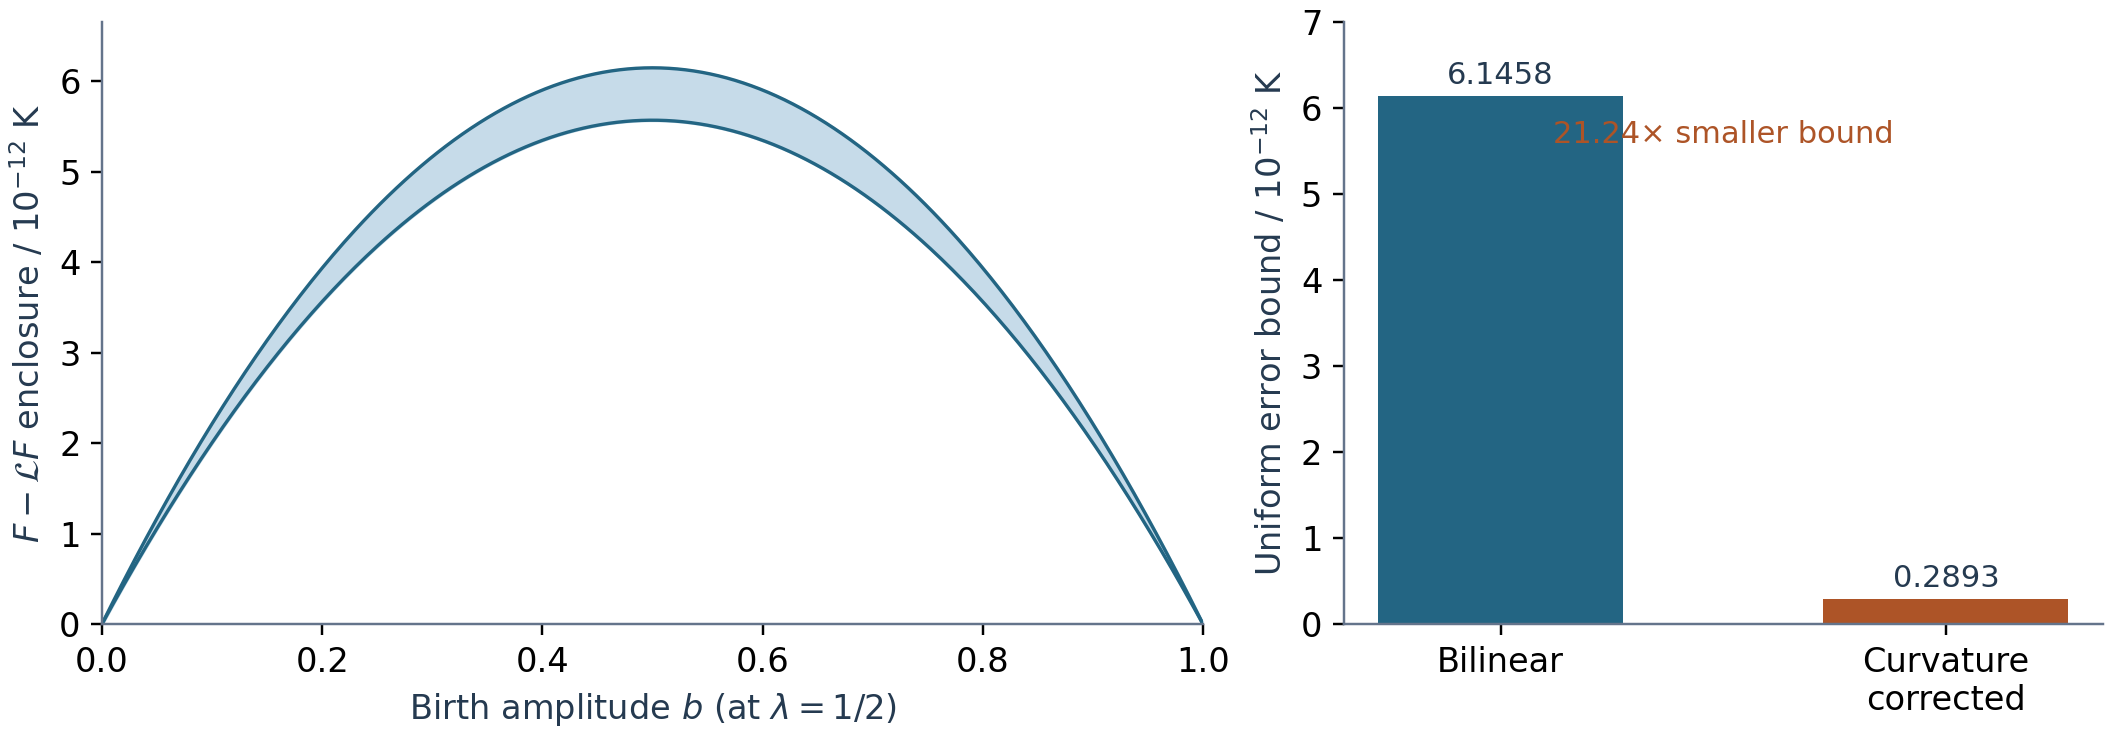
\includegraphics[width=0.98\textwidth]{figures/interpolation_error.png}
\caption{왼쪽: $\lambda=1/2$에서 인증된 bilinear 재구성의 signed error 포함.
오른쪽: 형상 재구성의 두 균일 상계 비교.
이는 계산된 inclusion 공식의 시각화이며, 물리 함수의 표본 시뮬레이션이 아니다.}
\end{figure}

\subsection{계수 해상도를 포함한 중심값 모델}
식 (19.23)--(19.26)은 실제 동일 계열 corner 계수를 유지한 형상 오차다.
수치 다항식을 얻으려면 $F_{00},a_\lambda,a_b,\mathcal I$도
구간 중심값으로 바꾸므로 그 계수 불확실성이 추가된다.
이 해상도를 함께 제시해야 유한 surrogate의 정확한 의미가 드러난다.

원 전체 온도 결함 포함을 $G$라 하자.
네 corner 모두 $G$에 속하므로
\[
[F_{00}]\leftarrow G\cap(G-[a_\lambda])\cap(G-[a_b])
\cap(G-[a_\lambda]-[a_b]-[\mathcal I])
\tag{19.28}
\]
로 안전하게 조일 수 있다.
원 $G=[-0.001585967387182,-0.001210819969055]\ {\rm K}$에서
다음 구간을 얻었다.
\begin{table}[H]\centering\small
\caption{실제 계수를 담는 외향 포함. 네 계수의 같은-family 관계는 유지한다.}
\begin{tabular}{ll}
\toprule
계수 & Kelvin 단위 포함\\
\midrule
$F_{00}$ & $[-0.001585959249676,-0.001278583452911]$\\
$a_\lambda$ & $[-1.009599125635,-0.8137506081166]10^{-8}$\\
$a_b$ & $[6.776348385589,7.185335549648]10^{-5}$\\
$\mathcal I$ & $[-2.668505746423,-2.118796636045]10^{-12}$\\
\bottomrule
\end{tabular}
\end{table}
각 중심을 $m_0,m_\lambda,m_b,m_I$, 반폭을 $r_0,r_\lambda,r_b,r_I$라 쓰고,
(19.27)을 사용한 수치 모델을
\[
P=m_0+m_\lambda\lambda+m_bb+m_I\lambda b
-\frac{c_A^{\rm dec}}2\lambda(1-\lambda)
-\frac{c_D^{\rm dec}}2b(1-b)
\]
로 정의한다.
$\widetilde r_A=\max_{a\in[A]}|a-c_A^{\rm dec}|$와
$\widetilde r_D$를 쓰면 점별 오차는
\[
\begin{aligned}
|F-P|\le{}&
r_0+r_\lambda\lambda+r_bb+r_I\lambda b\\
&+\frac{\widetilde r_A}{2}\lambda(1-\lambda)
+\frac{\widetilde r_D}{2}b(1-b).
\end{aligned}
\tag{19.29}
\]
따라서 이 전체 중심값 모델의 보수적인 균일 오차 상계는
\[
\boxed{\|F-P\|_\infty\le0.0001557338140092\ {\rm K}.}
\tag{19.30}
\]
모든 중심과 반폭은 정확한 유리수로 결과 JSON에 저장했다.
계수의 포함폭은 현재 family 정보의 해상도이며 실제 오차의 관측값은 아니다.
이를 줄이려면 특정한 $\alpha$와 실제 소비 상태를 결박한 추가 정보가 필요하다.
이번의 매우 작은 곡률 보정 오차는 그 다음 판단에 쓸 수 있는 재구성 부분을 닫아 준다.
